\documentclass[11pt,a4paper]{article}
\usepackage{fullpage}
\usepackage{times}
\usepackage{amsmath}
\usepackage{graphicx}
\usepackage{longtable}
\usepackage{supertabular}
\usepackage{tabularx}
\usepackage[]{ametsoc}
\bibliographystyle{ametsoc}

\begin{document}

\title{\centering \Huge \baselineskip30mm Introduction to UCLA-LES \\ \large Version 3.2.1}
\baselineskip7mm
\bigskip
\author{\LARGE Bjorn Stevens \\ } 
\maketitle

\baselineskip6mm

\newpage
\tableofcontents
\newpage

\normalsize
\section{Introduction}

\subsection{Distribution}
This code (the UCLA-LES) is free for all to use, distribute, and call
their own, following the guidelines of the gnu public license (http://www.gnu.org/licenses/).
The Code is distributed through git, a free software source code management project.
Subsequent developments of the code are available to its community here as well.
Please visit http://gitorious.org/uclales for more information.
[Referencing the origin of the code would also be appreciated. Relevant references in
this regard are \cite{Me:1999a,Me:2005b,Me:2008}.  These references
also document the behavior of the code for a variety of test-cases
developed in the context of the GEWEX Cloud Systems Studies Boundary
Layer Working Group.]
Users of the code assume full responsibility for the results they produce.
In addition users of the code are asked to share the burden of it's support.

\subsection{History and Contributions}
This code grew out of the cloud and meso-scale modeling projects
directed by Professors William R. Cotton and Roger Pielke in the
Department of Atmospheric Science at Colorado State University.
Most of the actual development in these projects was performed
by Craig Tremback, now of Mission Research Inc., Robert
L. Walko, now at Rutgers, Greg Tripoli, now at the University of
Wisconsin, and Jim Edwards, now at NCAR with IBM, their collective
efforts are reflected in many respects in this particular code --- a
descendant of the code they developed.  The actual development of this
code was mostly done by myself with important contributions by Jim
Edwards (the initial parallelization); Graham Feingold, Verica
Savic-Jovcic and Axel Seifert (microphysics); Hsin-Yuan Huang also has
implemented and tested a variety of subgrid models, which are not
incorporated in this distribution.

\section{Physical Model}
\subsection{Model Equations}

Prognostic variables include the three components of the wind
($u_i \equiv \{u,v,w\}$); the liquid-water potential
temperature, $\theta_l;$ the total-water mixing ratio, $q_t;$ and, as
the case may be, an arbitrary number of scalars, $\phi_m,$ in support
of microphysical processes, more sophisticated sub-grid models, or
studies of tracer transport or chemical processes. Grid-scale quantities
are denoted by an overbar. Roughly speaking they can be thought of as
grid-scale avaraged quantities where the exact term of the averaging
operator is implicitly defined by the numerics, and unknown.

The form of the equations solved by the model are (in tensor notation)
as follows:
\begin{eqnarray}
\frac{\partial \bar{u}_i}{\partial t} & = &- \bar{u}_j \,
\frac{\partial \bar{u}_i}{\partial x_j} - c_p \Theta_0 \frac{\partial
\bar{\pi}}{\partial x_i} + \, \frac{g \bar{\theta}_v ''}{\Theta_0} \,
\delta_{i3} \, + f_k (\bar{u}_j - V_{g,j}) \epsilon_{ijk} +
\frac{1}{\rho_0} \, \frac{\partial (\rho_0 \, \tau_{ij})} {\partial
x_j} ,
\label{eq:FM} \\
\frac{\partial \bar{\phi}}{\partial t} & = & - \bar{u}_j \,
\frac{\partial \, \bar{\phi}}{\partial x_j} + \frac{1}{\rho_0} \,
\frac{\partial (\rho_0 \, \gamma_{\phi j})} {\partial x_j} +
\frac{\partial F_{\phi}}{\partial x_j} \delta_{j3} ,
\label{eq:FTD}
\end{eqnarray}
subject to the anelastic continuity equation
\begin{equation}
\frac{\partial (\rho_0 u_i) }{\partial x_i} = 0 \label{eq:continuity}
\end{equation}
and an equation of state which we take to be the ideal gas law for
a perfect mixture:
\begin{equation}
\theta_v = \theta\left(1 + (R_v/R_d-1)q_t - (R_v/R_d)q_l\right).
\end{equation}

In the above $\bar{\pi}=(\bar{p}/p_{00})^{R_d/c_p}$ is the exner function,
it measures the dynamic pressure perturbation.
$F_\phi$ denotes a flux whose divergence contributes to the evolution
of $\phi$ (for instance radiation in the case $\phi = \theta_l$),
$f_k = \{0,0,f\}$ is the Coriolis parameter, $V_{g,j}$ is the
geostrophic wind, and
\begin{equation}
\tau_{ij} \equiv \overline{u_i u_j} - \bar{u}_i \bar{u}_j \quad
\text{and} \quad \gamma_{\phi j} \equiv \overline{\phi u_j} -
\bar{\phi} \bar{u}_j
\end{equation}
denote the sub-grid fluxes.  In (\ref{eq:FTD}) $\phi$ denotes an
arbitrary scalar.  Depending on the level of microphysical complexity
this can include $\theta_l$ and $q_t$ or an arbitrary number of
additional variables, for instance to represent microphysical habits
or categories.  The symbols $\delta_{jk}$ and $\epsilon_{ijk}$ denote
the Kronecker-delta and Levi-Civita symbol respectively.

The anelastic approximation solves for perturbations about a
hydrostatic basic state of constant potential temperature, i.e.,
\begin{equation}
\frac{d\pi_0}{dz} = -\frac{g}{c_p\Theta_0},
\end{equation}
where subscript $0$ denotes a basic state value, which depend only on
$z$ ($\Theta_0$ being constant). This follows the set of equation introduced by \cite{Ogura:1962}. Note that through the division by $\Theta_0$ in the buoyancy term, model results can be sensitive to the value chosen for $\Theta_0$.

In equation (\ref{eq:FM}) $\bar{\theta}_v''$
denotes the deviation of $\bar \theta_v$ from the basic-state $\Theta_0$. Thus, a mean
vertical acceleration can arise.  For consistency of the thermodynamic fields this requires the
introduction of a second pressure, $\pi_1:$
\begin{equation}
\frac{d}{dz}(\pi_0 + \pi_1) = -\frac{g}{c_p\bar{\theta_v}},
\end{equation}
that contains the contribution of deviations from the $\Theta_0$
reference state to the pressure.  This pressure depends on time, and
is updated in the code by finding the pressure that balances the mean
accelerations, such that
\begin{equation}
\frac{d\pi_1}{dz} = \frac{\dot{\overline{w}}}{c_p \Theta_0} ,
\end{equation}
with $\pi_1(z=0)$ fixed at its initial value.

The model represents the First Law of thermodynamics by (\ref{eq:FTD})
with $\phi=\theta_l.$  Where we define $\theta_l$ as:
\begin{equation}
\theta_l = T\pi \exp\left(-\frac{q_lL_v}{c_pT} \right)
\label{eq:thetal}
\end{equation} 
Hence the model satisfies an approximate form of the First Law, but
one generally consistent with the overall level of approximation. In
the above $L_v$, $R_d$, $R_v,$ $c_p$ and $p_{00}$ are thermodynamic
parameters which adopt standard values (see Table \ref{tbl:constants})
as is $g$ the gravitational acceleration.

\begin{table}[htb]
\caption{Default values of model constants} \label{tbl:constants}
\begin{center}
\begin{tabular}{cl}
Constant & Value \\ \hline \hline
$p_{00}$   & $10^5$   Pa \\
$R_d$      & 287.04 J kg$^{-1}$ K$^{-1}$ \\
$R_v$      & 461.5  J kg$^{-1}$ K$^{-1}$ \\
$c_p$      & 1004   J kg$^{-1}$ K$^{-1}$ \\
$L_v$      & 2.5 $\times 10 ^6$ J kg$^{-1}$ \\
$\Omega$   & 7.292 $\times 10 ^{-5}$ s$^{-1}$ \\
$g$        & 9.80 m s$^{-1}$ \\ \hline
\end{tabular}
\end{center}
\end{table}

The continuity equation (\ref{eq:continuity}), applied after taking
the density weighted divergence of (\ref{eq:FM}), yields $\tilde{\pi}$ through the
inversion of the Poisson equation:
\begin{equation}
\frac{\partial}{\partial x_i} \left( \rho_0 \frac{\partial
\tilde{\pi}}{\partial x_i} \right) = \frac{1}{c_p\Theta_0}
\left[\frac{\partial }{\partial x_i} \left ( - \rho_0 \bar{u}_j \,
\frac{\partial \bar{u}_i}{\partial x_j} + \, \frac{\rho_0 g
\bar{\theta}_v ''}{\Theta_0} \, \delta_{i3} \, + \rho_0 f_k (\bar{u}_j
- u_{jg}) \epsilon_{ijk} + \frac{\partial (\rho_0 \, \tau_{ij})}
{\partial x_j} \right ) \right],
\label{eq:FP}
\end{equation}

\subsection{Parameterizations and Models}

\subsubsection{Turbulence}

The sub-grid fluxes $\tau_{ij}$ and $\gamma_{\phi j}$ are not known
explicitly and thus must be modeled.  This constitutes the model
closure.  The basic or default form of the closure makes use of the
Smagorinsky model, wherein
\begin{equation}
\tau_{ij} = - \rho_0 K_mD_{ij} \quad \text{and} \quad \gamma_{\phi j}
= - \frac{K_m}{Pr} \frac{\partial \bar{\phi}} {\partial x_j},
\end{equation}
where \[D_{ij} = \frac{\partial \bar{u}_i}{\partial x_j} +
\frac{\partial \bar{u}_j}{\partial x_i}\] is the resolved deformation,
$K_m$ is the eddy viscosity, and $Pr$ is an eddy Prandtl number.  The
Smagorinsky model calculates the eddy viscosity as
\begin{equation}
K_m = (C_s \ell)^2 S \sqrt{1 - \frac{Ri}{Pr}} \quad \text{where} \quad
Ri =
\frac{S^2}{N^2}
\end{equation}
and
\begin{equation}
S^2 \equiv \frac{\partial \bar{u}_i}{\partial x_j} D_{ij} \quad
\text{and} \quad N^2 = \frac{g}{\Theta_0} \frac{\partial
\bar{\theta}_v}{\partial z}.
\end{equation}
In the above $C_s$ is the Smagorinsky constant and takes on values
near 0.2, and
\[ \ell^{-2} = (\Delta x \Delta y \Delta z)^{-2/3} + (z\kappa/C_s)^{-2},
\]  where $\kappa=0.35$ is the von K\'arm\'an constant in the model.   The
geometric averaging between a grid scale and a length scale proportional
to the height above the surface allows $K_m/(u_*z)$ to approach
$\kappa$ in the neutral surface layer (the log-law).

Other options include Lagrangian averaged scale-dependent and
scale-independent models (implemented by Hsin-Yuan Huang) the
Deardorff-Lilly sub-grid turbulence kinetic energy (TKE) model, and
for scalars the option of having all the dissipation carried by the
numerics.

\subsubsection{Microphysics}

The model allows for a range of microphysical complexity.  In the
standard distribution a warm-rain microphysical scheme is implemented
following the work of \cite{Seife:2001} as implemented in \cite{Me:2008}.
In this scheme cloud droplets are assumed to be in equilibrium with a fixed
(specified) concentration.  Cloud, or rain, drops defined as liquid
condensate with appreciable fall velocities are allowed to evolve
under the action of the ambient flow and microphysical processes
(auto-conversion, accretion, self-collection, sedimentation).  The
representation of these processes leads to the inclusion of two
additional prognostic equations, one for rain mass the other for rain
concentration.

A saturation adjustment scheme is also implemented in the model.
This scheme has no rain category and diagnoses cloud drop mass
concentrations by assuming homogeneity on the grid-scale and
equilibrium thermodynamics. Sedimentation of cloud droplets can
be implemented as a source term in the model, but is not a default.

The prognostic equations for the microphysical quantities used by the
bulk (level 3, imcrtyp 2) model, may be written as follows
\begin{equation}
\frac{\partial \psi}{\partial t} + \mathbf{u}\cdot \nabla\psi - \nabla
\cdot \left(K_\psi \nabla \psi \right)= -w_{\psi} \frac{\partial
\psi}{\partial z} + \mathcal{K}_{\psi} + \mathcal{T}_{\psi}
\label{eq:psi}
\end{equation}
where here $\psi$ stands for a microphysical variable, in our case
$\psi\in\{n_r,r_r\}$. The terms on the lhs represent dynamic
processes, and $K_{\psi}$ is the eddy diffusivity of $\psi$ which we
set to $K_h$ the eddy diffusivity of heat. The rhs terms represent
different classes of microphysical processes.  From left to right
these are: (i) sedimentation, with terminal velocity $w_\psi$; (ii)
$\mathcal{K}_\psi$, the transformation of $\psi$ due to kinetic
processes; and (iii) $\mathcal{T}_\psi,$ the transformation associated
with thermodynamic processes, which given our assumption that
condensation is carried entirely by the cloud droplets, includes only
evaporation.  Note that the microphysical literature often speaks of
kinetic effects in terms of molecular kinetics.  At the risk of
confusing matters, here we use \emph{kinetic} to describe
microphysical transformations arising from the interactions among
drops, namely effects associated with droplet collisions, such as
coalescence or breakup.

The Seifert and Beheng (SB) model is centered around the idea that the size distributions
of cloud droplets and rain drops can be described by separated
(truncated) gamma distributions with a separation diameter, $D_*$ of
80 microns.  The gamma distribution can be written as
\begin{equation}
f(D) = N_0 D^\mu \exp(-D/D_p),
\end{equation}
where $D_p,$ is the mean diameter, and $\mu$ is the shape parameter.
In the original formulation of the scheme cloud droplets were allowed
to have $\mu>0,$ while $\mu$ was fixed to zero for rain drops.  Here,
motivated by \cite{Seife:2008}, and the study
of \cite{Milbr:2005}, the formulation is generalized to allow $\mu >
0$ for the rain-drop mode as well.  Formally
\begin{equation}
n_r = \int_{D_*}^\infty f(D) \, \mathrm{d}D \quad \text{and} \quad r_r
= \frac{\rho_l\pi}{6} \int_{D_*}^\infty D^3 f(D) \, \mathrm{d}D
\end{equation}
where $D_*$ is the critical size separating drops from droplets, and
$\rho_l$ is the density of liquid water.  Given $f$, then the mean
volume (or mass) diameter follows as
\begin{equation}
D_m = \left[ \frac{1}{n_r} \int_{D_*}^\infty D^3 f(D) \right]^{1/3},
\end{equation}
and the mean diameter is
\begin{equation}
D_p = \frac{1}{n_r} \int_{D_*}^\infty D f(D)
\end{equation}
For a gamma distribution with $D_*=0$ the relationships among the
different microphysical moments, or parameters, depends only on $\mu,$
for instance
\begin{equation}
D_p = [\frac{6r_r}{\pi\rho_w
n_r}\frac{1}{(\mu+3)(\mu+2)(\mu+1)}]^{1/3} \quad \text{and}\quad N_0 =
\frac{n_r}{\Gamma(\mu+1)} D_p^{-(\mu+1)}.
\end{equation}
Because evaluating the integrals over $f(D)$ for $D_*\ne0$ yields
incomplete Gamma functions, which are computationally delicate to
represent, $D_*$ is often taken to zero when evaluating moments or
parameters of the droplet distribution.  In two-moment schemes $\mu$
usually enters as a parameter, although it can be allowed to vary as a
function of the other moments.  For instance, for many of our
simulations we diagnose
\begin{equation}
 \mu = 10(1 + \tanh(1200(D_m - 0.0014))) \label{eq:mu}
\end{equation}
so that for small $D_m$ the drop size distribution becomes
exponential.

Neglecting the effects of variable density (which can be justified for
shallow clouds, and is here done solely for to streamline the
discussion) the SB Model is as follows
\begin{eqnarray}
\mathcal{K}_{r_r}^{(sb)} & = & a_{sb} \frac{r_c^4}{N_c^2}
\phi_{cc}(\varepsilon) + b_{sb} r_cr_r
\phi_{cr}(\varepsilon)\label{eq:sb1} \\ \mathcal{K}_{n_r}^{(sb)} & = &
\frac{\rho_l \pi}{6} D_*^3\left(a_{sb} \frac{r_c^4}{N_c^2}
\phi_{cc}(\varepsilon) \right) - b_{sb} n_r r_r \beta(D_m). \label{eq:sbn}
\end{eqnarray}
Here $a_{sb}$ is a constant (Table~\ref{tbl:SB}) which is derived
using the \cite{Long:1974} Kernel for collection and incorporates the
assumed shape of the cloud-droplet distribution.  Collisional breakup
of raindrops, which includes rebound effects, \emph{i.e.,} all effects
of coalescence efficiencies less than unity, is represented by a
linear decrease of the self-collection rate, so that
\begin{equation}
\beta({D_m}) = \begin{cases} 1 & D_m \le 0.3 \times 10^{-3} \\
  1000D_m- 1.1 & D_m > 0.3  \times 10^{-3}\end{cases} .
\end{equation}
Non-equilibrium effects in auto-conversion and accretion are
respectively modeled by the terms
\begin{equation}
\phi_{cc}(\varepsilon) = 1 + 600 \frac{\varepsilon^{0.68} (
1-\varepsilon^{0.68})^3}{1-\varepsilon} \quad \text{and} \quad
\phi_{cr}(\varepsilon) = \left(\frac{\varepsilon}{\varepsilon + 5
\times 10^{-4}}\right)^4 \label{eq:phis}
\end{equation}
with 
\begin{equation}
\varepsilon = r_r/(r_c+r_r) \label{eq:epsilon}.
\end{equation}
Here $\varepsilon$ is to be thought of as a non-dimensional time that
measures the progression of the cloud water into rain water.  The
decomposition of the kinetic term into two additive terms is typical
for bulk models, whereby the first term is identified with a process
called auto-conversion, and the second represents accretion.
Auto-conversion in most models does not depend on $r_r.$ The $r_r$
dependency of the auto-conversion term of $\mathcal{K}^{(sb)},$
through the $\phi_{cc}$ term, attempts to represent the effects of
droplet spectral ripening \cite[]{Cotto:1972,Lupke:1989}.

Sedimentation in SB is determined through a specification of the
sedimentation velocities, which we write as
\begin{align}
& w_{n_r} = \frac{\int_{D_*}^\infty W_T(D) f(D) \,
\mathrm{d}D}{\int_{D_*}^\infty f(D) \, \mathrm{d}D} = 9.65[1 -
c_{sb}(1+600 D_p)^{-(\mu+1)} ] \label{eq:wn} \\
& w_{r_r} = \frac{\int_{D_*}^\infty W_T(D) D^3 f(D) \,
\mathrm{d}D}{\int_{D_*}^\infty D^3 f(D) \, \mathrm{d}D} =
9.65[1 - c_{sb}(1 + 600 D_p)^{-(\mu+4)} ],
\label{eq:wr}
\end{align}
where $W_T$ is the terminal velocity which depends only on the size of
the drop, and $c_{sb}$ is a constant, whose value along with other
constants used by the scheme are given in Table \ref{tbl:SB}. This
formulation differs from the original proposal of SB.

\begin{table}[htb]
\begin{center}
\caption{Constants for Microphysical Model. \label{tbl:SB}}
\begin{tabular}{ll} \hline \hline
Constant  & Values \\ \hline
$a_{sb}$  & $1.408 \, \times \, 10^{19}$ \\
$b_{sb}$  & 5.78 \\
$c_{sb}$  & 1.015113 \\ 
\end{tabular}
\end{center}
\end{table}

\subsubsection{Surface Fluxes}

\begin{table}[htb]
\caption{Similarity constants for surface layer.} \label{tbl:surface}
\begin{center}
\begin{tabular}{cl} \hline \hline
Constant & Value  \\ \hline
$Pr$       & 0.74 \\
$\kappa$   & 0.35 \\
$a_h$      & 7.8  \\
$a_m$      & 4.8  \\
$b_h$      & 12.0 \\
$b_m$      & 19.3 \\ \hline
\end{tabular}
\end{center}
\end{table}

To enforce the boundary conditions the model can either implement free
slip or no-slip boundary conditions on the grid-scale tangential
velocities, with free-slip being the default.  These grid-scale
quantities do however feel accelerations, or tendencies as a result of
sub-grid scale fluxes which are parameterized.  The model supports
different methodologies for specifying the sub-grid fluxes at the
lower boundary.  They can be prescribed, calculated based on
prescribed gradients, or prescribed surface properties.  For the
latter two similarity functions are chosen to relate the fluxes at the
surface to the grid-scale gradients there.  The similarity functions
used by the model are as follows:
\begin{eqnarray*}
\Phi_h & \equiv &\frac{\kappa z}{\theta_*} \left(\frac{\partial
\bar{\theta}}{\partial z}\right) = \begin{cases} Pr(1+a_h\zeta) &
\zeta > 0 \\ Pr(1-b_h\zeta)^{-1/2} & \zeta \le 0 \end{cases} \\ \Phi_m
& \equiv & \frac{\kappa z}{u_*} \left( \frac{\partial
\bar{u}}{\partial z} \right) = \begin{cases} (1+a_m\zeta) & \zeta > 0
\\ (1-b_m\zeta)^{-1/2} & \zeta \le 0 \end{cases}
\end{eqnarray*}
where
\[ \zeta = z/\lambda \quad \text{and} \quad \lambda =
\frac{\Theta_0}{g\kappa} \left(\frac{u_*^2}{\theta_*}\right) \] is the
Monin-Obukov length scale.  The similarity constants in this
formulation are listed in Table \ref{tbl:surface}.

\subsubsection{Radiation}
The model allows for a range of different radiation types.
As a default, calculations are done without
radiation (iradtyp=0). For more explicit radiation treatment one can either use
the simple radiation (iradtyp=2) following the gcss intercomparison or
the full radiation (iradtyp=4) from \cite{Pincus:2009}.
For simple radiation treatment, short- and longwave
radiation will be computed as described in \emph{src/rad\_gcss.f90}.
The full radiation package solves the radiative transfer with a delta-4 stream method.
A particular treatment
of radiation is available for the smoke cloud and the bellon
case. The radiation treatment for the smoke cloud case can be
used by setting iradtyp=2 and level=1. The bellon case has a
specific radiation code as shown in the bellon\_rad routine
and can be used by setting iradtyp=3.

\subsubsection{Land Surface Model}
The model can be used with an interactive land-surface scheme to calculate the fluxes between the land and atmosphere (isfctyp=5).
The scheme contains a surface layer and soil model following the approach used in the Dutch Atmospheric Large-Eddy Sumulation code \citep{Heus:2010}.
Fluxes are calculated solving the surface energy budget for each grid cell.
Below the surface, a four layer diffusive soil scheme is used to calculate temperature and soil moisture evolution in time.
A mean deep soil temperature is prescribed as a lower boundary of the model whereas the temperature and moisture of the surface and soil layers are evolving in time.
The land surface scheme can be used in combination with the full radiation package (iradtyp=4) following \cite{Pincus:2009}.
To assure a stable surface temperature the incoming long and shortwave radiation is averaged over a number of time steps.
The interactive calculation of latent and sensible heat fluxes allows for multiple feedbacks in the coupled land-atmosphere system.
This land surface setup has been tested against the Dutch Atmospheric LES (DALES) in a dry convective environment.
To run the model with the interactive land-surface scheme an additional Namelist (SURFNAMELIST) is needed to specify surface and soil settings, which can be found in the \emph{misc} directory.

\subsubsection{Lagrangian Particle Tracking}
The Lagrangian particle tracking module is described in a separate document (LPTM\_doc), located within the same directory as this LES documentation.

\section{Numerics}

\subsection{Time-stepping}
Time stepping is based on a Runge-Kutta third order method.
An iterative method for the approximation of differential equations.
A new timestep is computed using weighted supporting points (tendencies) for the calculation.
The substeps done to determine any variable ($\phi$) at the next timestep ($\phi^{n+1}$) are
calculated according to equations (\ref{eq:phi1})-(\ref{eq:phi3}).
The weighting factors are set to be $\alpha_i = (\frac{8}{15}, -\frac{17}{60}, \frac{3}{4})$
and $\beta_i = (0, -\frac{15}{12}, -\frac{15}{12})$. 

\begin{equation}
	\phi_*^{n} = \phi^{n} + \alpha_1 \frac{\partial \phi^{n}}{\partial t} \Delta t \\
	\label{eq:phi1}
\end{equation}

\begin{equation}
	\phi_{**}^{n} = \phi_*^{n} + \alpha_2 \frac{\partial \phi^{n}}{\partial t} \Delta t + \beta_2 \frac{\partial \phi_*^{n}}{\partial t} \Delta t\\
	\label{eq:phi2}
\end{equation}

\begin{equation}
	\phi^{n+1} = \phi_{**}^{n} + \alpha_3 \frac{\partial \phi_{**}^{n}}{\partial t} \Delta t + \beta_3 \frac{\partial \phi_*^{n}}{\partial t} \Delta t\\
	\label{eq:phi3}
\end{equation}

The model employs a variable timestep, which is set so as to maintain
a constant CFL maximum value bounded above by the value of the maximum
timestep (dtlong in the NAMELIST file). If dtlong exceeds the maximum
CFL value the actual timestep is scaled so that CFL value according
to the new timestep is always 0.5.

\subsection{Computational Grid}
\begin{figure}[htb]
\centering \leavevmode 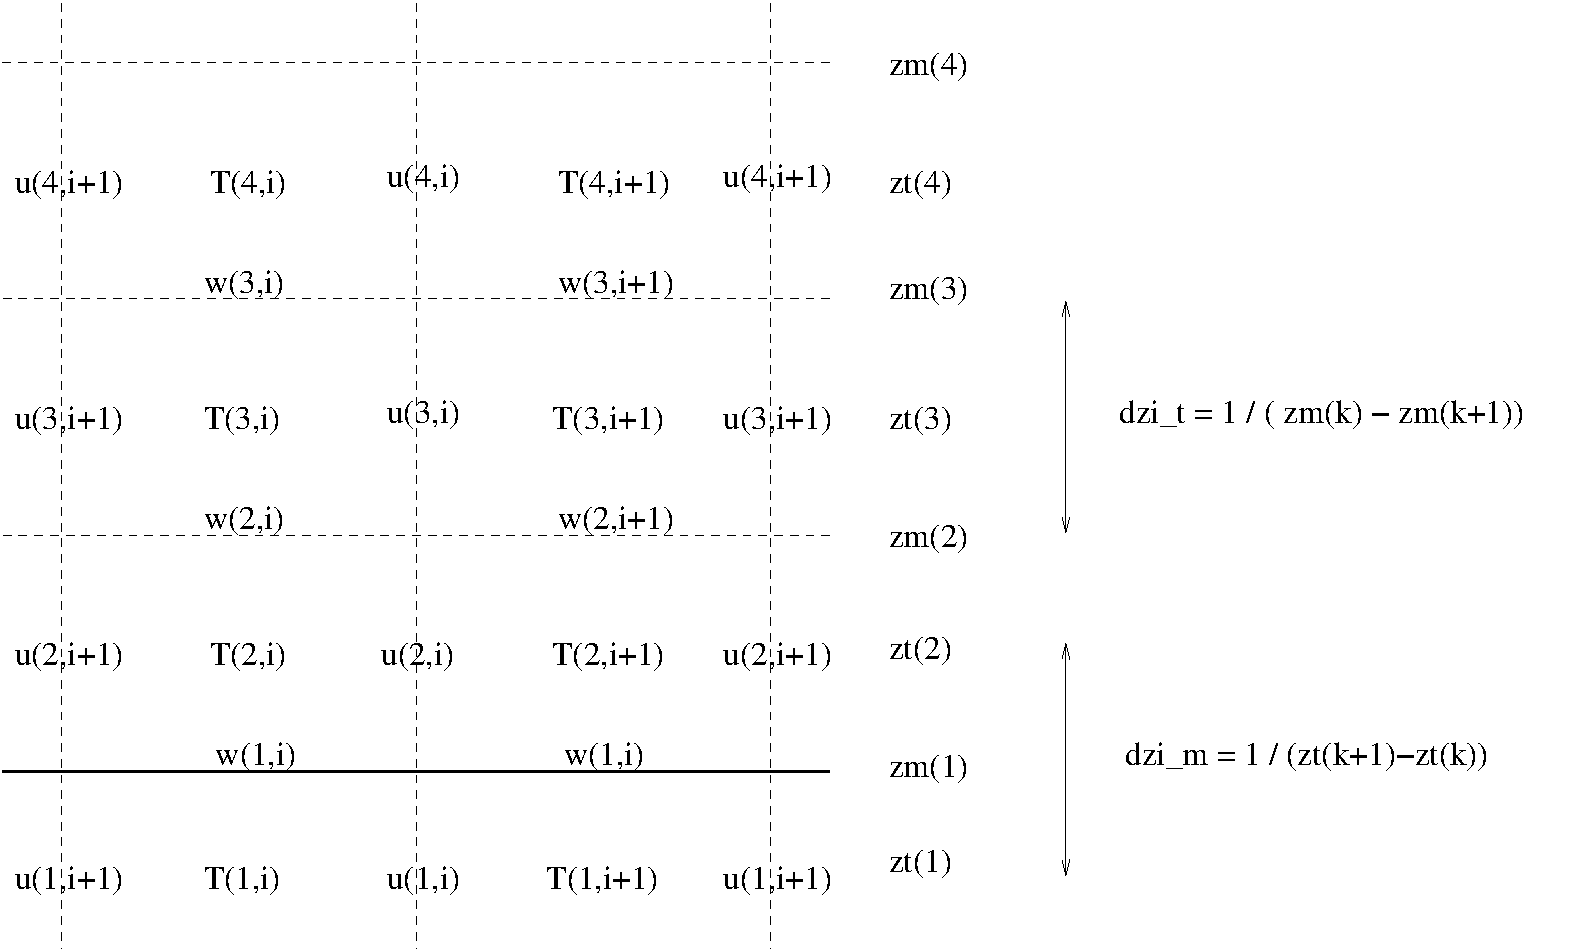
\includegraphics[width=12cm]{grid2}
\caption{Schematic depiction of the model grid and where variables
locate on it.}
\label{fig:grid}
\end{figure}

The grid is doubly periodic (in $x$-$y$) and bounded in the vertical,
$z.$ The vertical is spanned by a stretchable grid, the horizontal is
tiled by uniform squares. Scalar advection is based on a
directional-split monotone up winding method while momentum advection
uses directionally-split fourth-order centered differences.
The model uses the Arakawa-C grid, which means that $u(k,i,j)$ lies
$\frac{\Delta x}{2} $ meters to the right of $\theta_l(k,i,j)$. To
state this more generally, velocities are staggered half a grid point
up-grid (in the direction of the specific velocity component) of the
thermodynamic and pressure points.  Also note that the grid indexing
has the z dimension first.\footnote{Although given the way the model
is written, this is merely a social contract among the various
subroutines and thus could be changed.}  This $k,i,j$ indexing is
chosen in realization of the fact that many of the operations in the
model are done column-wise.  The grid configuration, and some height
variables that are commonly used in the code (i.e., \it zm, zt, dzm=dzi\_m,
\rm and \it dzt=dzi\_t \rm) are illustrated in a schematic drawing in
Fig.~\ref{fig:grid}.

\subsection{Pressure Solver}
Pressure is solved by a fractional step method so as to ensure that
the velocities at the end of the timestep satisfy
(\ref{eq:continuity}) to machine accuracy.  The solver takes
advantage of the periodicity in the horizontal to use 2-D FFTs to
transform the Poisson-equation to a second order ODE in the
vertical. Schematically
\begin{equation}
\frac{\partial^2 \pi}{\partial x_i^2} \longrightarrow
(k^2+l^2)\frac{d^2\pi}{dz^2},
\end{equation}
where $k$ and $l$ denote the horizontal wave-numbers.  The resultant
ODE is then solved using a tri-diagnonal solver.

\subsection{Parallelization Strategy}

\paragraph{Decomposition}

The parallelization is performed by decomposing the domain into
sub-domains consisting of columns in the $x$-$y$ plane. This is
a 2D decomposition in that the parallelization is along both the
$x$ and $y$ dimensions. What results is $N_p$ $x$-$y$ columns
where the number of grid points is evenly divided over the processors.
$N_p$ denotes the number of processors (columns) and $N_x$ and $N_y$
are the total number of unique $x$- and $y$-points. The way the
memory is organized this has almost no impact on the code but
requires that the columns have at least two unique $x$ and $y$
points. It also allows us to use domain-independent indexing,
so that $j \in \{1,\ldots,N_y/N_p+4\}$ where $j$ is the $y-$index.
The addend of four represents the contribution from the ghost points.
The width of the ghost-points depends on the size of the largest
stencil used for a differencing computation in the code.
In our case the fourth order differences in the treatment of momentum
fluxes. The effect of the ghost-strips is to increase the number of
grid-points at the boundaries of the domain. This is required to
calculate derivatives with the fourth order differences method as an
example. The total number of grid-points, $N_t$ is thus processor dependent.
\\
\\
2D parallelization allows us in principle to use $N_xN_y/4$
processors, i.e., more than 4 million with $N_x=N_y=4096$.
The normalized computational overhead associated with the ghost points
can be measured by forming the ratio $R(N_p) = N_t(N_p)/N_t(1)$.
For 2D decomposition with 2 ghost points deep:
\[R(N_p) = 1 + \frac{16(N_p-1) + 4(N_x+N_y)\sqrt{N_p}}{N_xN_y + 16} \]
For $N_x = N_y = 2\sqrt{N_p} \gg 1$ this ratio approaches 7, although
the communication overhead of such a large computation is more likely
to be the bottleneck. I/O is currently handled by each processor.

\paragraph{Communication}
With the current 2-D parallelization strategy global communications
are needed to implement boundary conditions, compute domain
integrals (such as means and co-variances), and calculate the FFTs.
The latter is the most significant issue. The domain is first redistributed
into strips (x-z plane).FFTs are computed in the $x-$direction (along a strip),
then the domain is transposed into strips in the $y-$direction.
After the transpose the FFTs are computed in the $y$-direction and
then the vertical solver (tri-diagonal) solves the ODE (over $z$) in
the transpose space.  The inverse FFTs are then done in this transpose
space, then the inverse transpose is performed before computing the
inverse FFT along the strips in the $x$-direction.  This strategy only
requires four global communications per solve.

\section{The Code}
\subsection{Getting the Code}
The UCLA-LES Code is free for all to use, distribute, and call their own,
following the guidelines of the gnu public license (http://www.gnu.org/licenses/).
It is distributed through git, a free software source code management project.
Subsequent developments of the code are available to its community here as well.
The newest version of UCLA-LES will always be available at \textbf{http://git.gitorious.org/uclales}.
To Download the newest UCLA-LES version make sure you have git installed on your system.
Typing ``git clone git@gitorious.org:uclales/uclales.git'' in the command line
will download the sources. You may want to check for updates by typing ``git pull ''
in the command line. To check what has been changed since the last commit use
``git status'' and ``git diff''. You can also insert your private UCLA-LES version into git.
For further information visit http://git.gitorious.org/uclales and see the git\_uclales document
in \emph{doc} directory. Users of the code assume full responsibility for the results they produce.
In addition users of the code are asked to share the burden of it's support.

\subsection{Organization}

The basic model is configured to solve an anelastic system of
equations on the $f$-plane.  It is written in F90/95, and is
parallelized using a two-dimensional decomposition and MPI.  Its
primary form of output is NetCDF files, with FORTRAN binary output of
history and restart files. The distribution is spread among four
directories: \emph{bin}, \emph{doc}, \emph{misc} and \emph{src}.
The code itself resides in \emph{src} and is organized in F90 modules.
These are described in Table~\ref{tbl:modules}.
This directory also contains two subdirectories \emph{seq} and \emph{mpi}
where the sequential or MPI modules are stored upon compilation. In addition
rfft.F contains the Swartztrauber FFT routines which are called from
the util module. Lastly a Makefile here formed by the master Makefile
in \emph{bin} defines the specific compilation/archive rules.
To add new modules requires modification of this makefile.

The \emph{bin} directory contains job control scripts and Makefiles
which have to be adjusted to machine standards. The model is compiled
from this directory (usually by typing make mpi or make seq respectively)
and typically executed from here as well. The file NAMELIST defines any
non-default input and is therefore the main control file.

The \emph{doc} directory contains the latest version of this documentation.
Also the gnu public license (also available at http://www.gnu.org/licenses/) which
concerns the use of this UCLA-LES code can be found here. As described earlier the
UCLA-LES is distributed through git. Here the git\_uclales document gives an introduction
how to use it in detail.

The \emph{misc} directory is a catchall for other useful things, for instance 
\emph{misc/initfiles} contains several NAMELIST files for idealized cases.
Makefiles and jobscripts can be found in \emph{misc/makefiles} and 
\emph{misc/initfiles} respectively. \emph{misc/synthesis} as well as
\emph{misc/scripts} contain other useful scripts.
To start postprocessing \emph{misc/analysis} suggests some simple NCL
(the NCAR Command Language) scripts for plotting. NCL is a powerful
data analysis , visualization, file-handling scripting language that
is free and distributed by NCAR (National Center Of Atmospheric Research).

\begin{table}
\begin{center}
\caption{Module F90 Files in \emph{src} directory} \label{tbl:modules}
\begin{tabular}[htb]{p{0.15\linewidth}p{0.85\linewidth}}
\hline \hline Module & Contains \\ \\  \hline
LES &  Main program which calls a timing
routine and the driver, as well as the driver subroutine and the
subroutine which defines and reads the model NAMELIST file. 
\\ advf &  Calculates the tendencies associated with scalar advection.
\\ advl &  Calculates the tendencies associated with momentum advection.
\\ defs &  Defines physical constants.
\\ forc &  Case specific forcings (radiation, subsidence, \emph{etc.}).
\\ grid &  Definition of grid, allocation of memory and I/O management
\\ init &  Routines for processing input (either from
a file or the NAMELIST), definition of basic state, initialization of
fields, and definition of initial random perturbations.
\\ lsvar &  computes sst, div and winds for astex case (only when lsvar=true in NAMELIST)
\\ ncio &  Defines structure of ncdf output files.
\\ mcrp &  Bulk microphysical routines.
\\ mpi\_interface & Definition of MPI parameters and MPI
routines for the domain decomposition (only when using MPI mode else seq\_interface).
\\ prss &  Poisson solver, calculates the velocity tendencies
associated with pressure gradients, also implements time-filter for
leapfrog scheme and updates velocity.
\\ rad\_cldwtr & Calculates radiation properties from cloud water and effective radius.
\\ rad\_corkds & Reads gas concentrations and calculates radiative properties such as optical depth and absorption coefficients.
\\ rad\_d4strm & Computes radiative fluxes and optical properties for Rayleigh scattering.
\\ rad\_driver & Includes background soundings for atmospheric gases.
\\ rad\_gcss & Simple radiative parametrization for SW and LW fluxes (Delta-Eddigton approximation).
\\ rad\_rndnmb & Contains a random number generator.
\\ rad\_solver & Radiation solver.
\\ sgsm &  Subgrid scale solver.
\\ srfc &  Surface boundary condition routines.
\\ stat &  Routines for calculating, accumulating and outputting model
statistics.  Statistical output is provided through the course of a
simulation and tends to be problem specific.
\\ step &  Time stepper.  Also includes several routines for computing
tendencies due to physical processes (Coriolis force, buoyancy) or
boundary conditions (Rayleigh friction for sponge layer near lid).
Updating of scalars is done here. CFL computations and
timestep-regridding are also here.
\\ thrm & Thermodynamic routines for calculating
quantities like temperature, and cloud water, given the thermodynamic
state of the model, i.e., $\theta_l,q_t,\rho_0,\pi_0,\Theta_0.$
\\ util & A collection of basic utilities including
boundary conditions, FFT calls, explicit array operations such as
domain or slab averaging or covariances, the tri-diagonal solver, and
some NetCDF utilities.  Many of the routines in this module make
active MPI calls.\\ \hline \hline
\end{tabular}
\end{center}
\end{table}

\subsection{Compilation}
There are two ways of compiling the code: The preferred way uses CMake. CMake aims to resolve dependencies and compilation sequence automatically, allows for parallel compilation, and for quick switching between compilers or between debug and release mode.
If CMake is not available on the system, some older example Makefiles are also provided.

\subsubsection{CMake}
The first thing to setup is a config file with the paths to the various libraries. CMake will try to find the libraries on its own, but on many clusters the paths are non-standard, so we need to provide some pointers. Example files are available in the \emph{config} directory. If any of these \emph{*.cmake} files matches your system, copy it to \emph{default.cmake} (still in the \emph{config} dir). If not, modify any of the files to create your own \emph{default.cmake}. 

Next thing is to create a build directory from where we will compile the code: \emph{mkdir build \&\& cd build} from the root dir of the code. To configure the code call cmake: \emph{cmake ..} where ``..'' is the path back to the root directory of the code. After this, the code can be build with \emph{make -j 4}, to use 4 processors while building the code. The resulting \emph{uclales} binary can then be found in the \emph{build} directory.

Changing from release mode (the default) to debug mode (with debug info, more restrictive checks, and less optimization) can be done with a cmake command line option: \mbox{\emph{cmake -D CMAKE\_BUILD\_TYPE=DEBUG ..}} and \mbox{\emph{cmake -D CMAKE\_BUILD\_TYPE=RELEASE ..}} respectively. Note that these options are persistent in that they will stay put for all compiling rounds, until being changed again by a cmake command.

\subsubsection{Make}
To compile the model type ``make'' in the the 
\emph{bin} directory. This will build the default version of the model using the default
architecture. To compile the code on different machines \emph{bin/Makefile} 
must be adjusted. Examples of Makefiles are stored in \emph{misc/makefiles}.
Currently there are settings to compile on IBM, Macs with IBM/Motorola processors 
and the XLF compiler, and Linux. The code compiles and runs with G95 but our
experiences to date with this compiler suggest that it produces
executable which is a factor of two or more slower than commodity
compilers.

The model requires the NetCDF libraries to build, and where they
locate needs to be specified in \emph{bin.}  Our experiences with the
most aggressive optimization has been generally positive on the IBMs,
less so on the Mac.  Fine tuning the optimization can lead to
performance gains of 50\% or more, but aggressive optimisation (O3 or
greater on XLF compilers) should be checked.  For computations with
more than 128 points in a horizontal direction the code should be
promoted to double precision, if only to yield better defined global
integrals.  One such integral that ends up being important is the mean
buoyancy which must be subtracted from the local buoyancy so as to not
cause any mean accelerations.

\subsection{Specialized model configurations}
Perhaps the best way to learn how to configure the model for different
problems is to look at the configuration templates in the \emph{misc}
directories.  Here sub-directories (\emph{e.g.,} cumulus, gcss\_dycoms,
etc.,) contain substitute forcing, statistical and other modules, as
well as alternate NAMELIST files.  These are designed to run specific
past cases and produce output required by them.  Looking over how this
is done in the code could provide an example of how to set up your own
case, and statistical output.  Starting from a case that is close to
your desired objectives would naturally be the most straightforward
way to proceed.

\section{Running the Model}
To run the model simply type the name of the executable (usually les.seq
for sequential or les.mpi for parallel execution), otherwise one can 
submit it using a batch scheduler. The latter is almost always
necessary in parallel programming environments. Runscripts to
schedule the job using IBM Loadleveler or IBM Load Sharing protocols
are provided in the \emph{misc/jobscripts} directory.

\subsection{The NAMELIST}
Model execution can be controlled by NAMELIST parameters. If a
NAMELIST parameter does not appear in the NAMELIST file for a
particular instance of the model execution, then the default value for that
variable is assumed.  In Table \ref{tbl:namelist} we list the NAMELIST
variables, their default values, the module in which they locate, and
specialized behavior which can be obtained by specifying non-standard
NAMELIST values.
\\
The execution is controlled by a number of model parameters which are
given default specifications in the code. These specifications can be
modified in the NAMELIST file so as to allow multiple execution
without recompilation.  The full NAMELIST is defined in the LES.F90
subroutine and is described, along with default parameter values, in Table \ref{tbl:namelist}. 

\clearpage

\begin{longtable}[htb]{p{0.12\linewidth}p{0.1\linewidth}p{0.18\linewidth}p{0.5\linewidth}}
\caption{NAMELIST variables and default values}\\
\hline
\hline
Variable & Module & Default Value & Comments \\ 
\hline
\endhead
nxp          & grid & 132                 & total number of $x$ points ($N_y+4$)                  \\
nyp          &  ''  & 132                 & total number of $y$ points ($N_y+4$)                  \\
nzp          &  ''  & 105                 & total number of $z$ points                            \\
nxpart       &  ''  & true                & 2D domain decomposition                               \\
deltax       &  ''  & 35.0 m              & grid spacing in $x$-direction                         \\
deltay       &  ''  & 35.0 m              & grid spacing in $y$-direction                         \\
deltaz       &  ''  & 17.5 m              & grid spacing in $z$-direction                         \\
dzrat        &  ''  & 1.0                 & grid stretching ration                                \\
dzmax        &  ''  & 1200 m              & height at which grid-stretching begins                \\
dtlong       &  ''  & 10 s                & maximum timestep                                      \\
nfpt         &  ''  & 10                  & number of levels in upper sponge layer                \\
distim       &  ''  & 300 s               & minimum relaxation time in sponge layer               \\
th00         &  ''  & 288                 & basic state potential temperature                     \\
igrdtyp      &  ''  & 1                   & control parameter for selecting vertical grid         \\
             &      &                     & \hspace{2mm} 1 = using nzp, deltaz, dzrat, dzmax      \\
             &      &                     & \hspace{2mm} 2 = Tschebyschev grid                    \\
             &      &                     & \hspace{2mm} 3 = grid supplied via zm\_grid\_in       \\
iradtyp      &  ''  & 0                   & control parameter for selecting radiation model       \\
             &      &                     & \hspace{2mm} 1,2,3 = case specific (see forc.f90)     \\
             &      &                     & \hspace{2mm} 4     = delta-4 stream radiative transfer\\
             &      &                     & \hspace{2mm} 5     = surface radiation                \\
lrad\_ca     &  ''  & false               & Perform clear air radiation calculations              \\              
isfctyp      &  ''  & 0                   & control parameter for surface type                    \\
             &      &                     & \hspace{2mm} 0 = prescribed fluxes in dthcon, drtcon  \\
             &      &                     & \hspace{2mm} 1 = prescribed gradient in dthcon, drtcon\\
             &      &                     & \hspace{2mm} 2 = sea surface ($q_{surf} = q_{sat}(SST)$ \\
             &      &                     & \hspace{2mm} 3 = sea surface ?                        \\
             &      &                     & \hspace{2mm} 4 = Variable $T_{surface}$ for constant buoyancy flux \\
             &      &                     & \hspace{2mm} 5 = Interactive land surface scheme      \\
sfc\_albedo  &  ''  & 0.05                & Surface albedo                                        \\
naddsc       &  ''  & 0                   & number of additional scalars                          \\
CCN          &  ''  & 150 $\times 10^{6}$ & cloud droplet mixing ratio                            \\
expnme       &  ''  & Default             & experiment name                                       \\
filprf       &  ''  & x                   & file prefix for use in constructing output files      \\
runtype      &  ''  & INITIAL             & type of run ('INITIAL' or 'HISTORY')                  \\ 
level        &  ''  & 0                   & \hspace{2mm} 0 = heat ($\theta$) only                 \\ 
             &      &                     & \hspace{2mm} 1 = + water vapor ($q_v$)                \\
             &      &                     & \hspace{2mm} 2 = + liquid water ($q_l$)               \\
             &      &                     & \hspace{2mm} 3 = + rain ($q_r$)                       \\
             &      &                     & \hspace{2mm} 4 = + ice, snow, graupel ($q_i,q_s,q_g$) \\
             &      &                     & \hspace{2mm} 5 = + two-moment scheme                  \\
umean        &  ''  & 0 m/s               & Galilean transformation                               \\ 
vmean        &  ''  & 0 m/s               & Galilean transformation                               \\ 
lcouvreux    &  ''  & false               & Couvreux decaying scalar                              \\
lwaterbudget &  ''  & false               & Liquid water budget diagnostics (level=3)             \\
\hline
ipsflg       & init & 1                   & control parameter for input sounding \textit{ps}      \\
             &      &                     & \hspace{2mm} 0 = pressure in hPa                      \\
             &      &                     & \hspace{2mm} 1 = meters, with ps(1) = $p_{sfc}$       \\
itsflg       &  ''  & 1                   & control parameter for input sounding \textit{ts}      \\ 
             &      &                     & \hspace{2mm} 0 = $\theta$, 1 = $\theta_l$             \\
irsflg       &  ''  & 1                   & control parameter for input sounding \textit{rts}     \\
             &      &                     & \hspace{2mm} 0 = $q_t$ calculated from RH provided in \textit{rts} \\
             &      &                     & \hspace{2mm} 1 = input \textit{rts} in $g \ kg^{-1}$  \\
us           &  ''  & n/a                 & input zonal wind sounding (max 500 points)            \\
vs           &  ''  & n/a                 & input meridional wind sounding (max 500 points)       \\
ts           &  ''  & n/a                 & input temperature sounding (max 500 points)           \\
rts          &  ''  & n/a                 & input humidity sounding (max 500 points)              \\
ps           &  ''  & n/a                 & input pressure sounding (max 500 points)              \\
iseed        &  ''  & 0                   & random seed                                           \\
zrand        &  ''  & 200 m               & height below which random perturbations are added     \\
mag\_pert\_t &  ''  & 0.2 K               & magnitude of temperature pertubations                 \\
mag\_pert\_q &  ''  & 5 $\times 10^{-5} kg / kg^{-1}$ & magnitude of moisture pertubations        \\
hfilin       &  ''  & test.               & name of input history file for HISTORY starts (xxx.)  \\
lhomrestart  &  ''  & false               & homogenize fields after restart                       \\
\hline
timmax       & step & 18000 s             & final time of simulation                              \\ 
wctime       &  ''  & 1e10 s              & wall-clock limit                                      \\
frqhis       &  ''  & 9000 s              & history write interval                                \\
frqanl       &  ''  & 3600 s              & analysis write interval                               \\
frqcross     &  ''  & 3600 s              & cross section write interval                          \\
istpfl       &  ''  & 1                   & print interval for timestep info                      \\
corflg       &  ''  & false               & coriolis acceleration                                 \\
radfrq       &  ''  & 0                   & radiation update interval                             \\
strtim       &  ''  & 0                   & UTC of model time                                     \\
cntlat       &  ''  & 31.5$^{\circ}$ N    & model central latitude                                \\
case\_name   &  ''  & astex               & specify case name (rico, astex, bomex, ..)            \\
lsvarflg     &  ''  & false               & reads large scale forcings from the file lscale\_in   \\
div          &  ''  & 0 s$^{-1}$          & divergence                                            \\
sst          &  ''  & 292 K               & (sea) surface temperature                             \\ 
lanom        &  ''  & false               & ...                                                   \\
tau          &  ''  & 900 s               & decay time scale Couvreux scalar                      \\
\hline
ltimedep     & modtimedep & false         & time dependant surface and large scale forcings       \\ 
\hline
lstendflg    & forc & false               & large scale advective tendencies (file lstend\_in)    \\
\hline
lmtr         & advf & 3                   & limiter in flux-limited scalar advection              \\ 
             &      &                     & \hspace{2mm} 0=no limiter, 1=minmod, 2=superbee       \\
             &      &                     & \hspace{2mm} 3=mc, 4=van leer                         \\
\hline
advm         & advl & 4                   & momentum advection scheme                             \\ 
             &      &                     & \hspace{2mm} 2=2nd order centered                     \\
             &      &                     & \hspace{2mm} 4=2nd order centered                     \\
\hline
csx          & sgsm & 0.23                & Smagorinsky Coefficient                               \\
prndtl       &  ''  & 1/3                 & Prandtl Number (if less than zero no sgsm for scalars) \\
clouddiff    &  ''  & -1                  & Additional diffusion outside clouds                   \\
\hline
ubmin        & srfc & 0.20                & minimum $u$ for $u_*$ computation                     \\
zrough       &  ''  & 0.01                & momentum roughness height (if less than zero use Charnock relation) \\
dthcon       &  ''  & 100 Wm$^{-2}$       & itsflg=0: surface sensible heat flux                  \\
             &      &                     & itsflg=1: surface temperature gradient                \\
drtcon       &  ''  & 0   Wm$^{-2}$       & itsflg=0: surface latent heat flux                    \\
             &      &                     & itsflg=1: surface mixing-ratio gradient               \\
rh\_srf      &  ''  & 1.                  & surface relative humidity                             \\ 
drag         &  ''  & -1                  & optional prescribed drag coefficient                  \\
lhomflx      &  ''  & false               & homogenize surface fluxes                             \\ 
\hline
fixed\_sun   &rad\_driver& false          & fix solar zenith angle                                \\
u0           &  ''  & n/a                 & cos(solar zenith angle) for fixed\_sun=true           \\
rad\_eff\_radius & '' & 1                 & fix for the cloud drop effective radius \\
\hline
cloud\_type  & mcrp & 2403                & Icemicro settings      \\
lrandommicro &  ''  & false               & Do the microphysical terms in random order or not                                 \\
microseq     &  ''  & \{1,2,..,23\}       & Specify the order of the microphysical terms      \\
timenuc      &  ''  & 60                  & Ice nucleation time scale                                   \\
nin\_set     &  ''  & 1700                & Ice nuclei number  \\
lpartdrop    &  ''  & false               & ...                                                   \\
\hline
SolarConstant& defs & 1365 $Wm^{-1}$      & Solar constant                                        \\ 
\hline
ssam\_intvl  & stat & 30 s                & statistics sampling interval                          \\
savg\_intvl  &  ''  & 1800 s              & statistics averaging interval                         \\
\hline
lcross       & modcross & false              & cross sections                                     \\
lxy          &  ''  & false               & xy output                                             \\
lxz          &  ''  & false               & xz output                                             \\
lyz          &  ''  & false               & yz output                                             \\
xcross       &  ''  & 0 m                 & location of x slice                                   \\
ycross       &  ''  & 0 m                 & location of y slice                                   \\
zcross       &  ''  & 0 m                 & location of z slice (max 10 points, z$>$0), or:       \\
             &      &                     & \hspace{2mm} -1 = at height maximum buoyancy variance \\
             &      &                     & \hspace{2mm} -2 = at cloud base                       \\
             &      &                     & \hspace{2mm} -3 = at lifting condensation level       \\
crossvars    &  ''  & see modcross.f90    & list of output variables                              \\
prc\_lev     &  ''  & -1                  & Output levels for the precip crosssections     \\

\hline
lpartic      & particles & false          & Lagrangian particles                                  \\
lpartsgs     &  ''  & false               & sub-grid scheme particles                             \\
lrandsurf    &  ''  & false               & randomize particles near surface                      \\
lpartstat    &  ''  & false               & bin-average particle statistics                       \\
lpartdump    &  ''  & false               & raw (netcdf) particle analysis files                  \\
frqpartdump  &  ''  & 3600 s              & frequency of writing analysis files                   \\                
lpartdumpui  &  ''  & false               & write velocities to analysis                          \\
lpartdumpth  &  ''  & false               & write potential temperatures to analysis              \\
lpartdumpmr  &  ''  & false               & write mixing ratios to analysis                       \\
ldropstart   &  ''  & 0 s                 & ...                                                   \\
\hline
lsync        & modnetcdf & false          & switch for buffering or immediate (much slower) IO in the netcdf files \\
deflate\_level&  ''  & 0                  & NetCDF compression factor                             \\
\hline
lnudge       & modnudge & false           & nudging of wind and scalars to predefined profiles    \\ 
tnudgefac    &  ''  & 1                   & nudging time scale                                    \\
qfloor       &  ''  & -1                  & (CGILS parameter) below zfloor, qt will be kept above this value \\
zfloor       &  ''  & 1200 m              & (CGILS parameter) below this value, qt will be kept above qfloor                                    \\
znudgemin    &  ''  & -1                  & lower bound of the transition layer between free development and nudged atmoshpere \\
znudgeplus   &  ''  & -1                  & upper bound of the transition layer between free development and nudged atmoshpere \\
lnudgebound  &  ''  & false               & ...                                                   \\
\hline
\hline
\label{tbl:namelist}
\end{longtable}
To run a specific case one can copy the appropriate NAMELIST from
\emph{misc/initfiles} (see list of available NAMELIST files below).
One may want to adjust parameters such as e.g. filprf, dtime,
timmax, iradtyp,level and others before running the model.
Here the use of the NAMELIST allows to change properties
without recompiling the model. As an example, the parameter
case\_name in the NAMELIST file can be used to set large scale
forcings for a specific case. Currently available case\_names
are: rico, bomex and atex.

\begin{itemize}
\item \textbf{namelist\_astex}: The Astex case.
\item \textbf{namelist\_cumulus}: Namelist to reproduce the idealized
cumulus cases reported in Stevens, JAS (2007). Requires the
generation of a sound\_in file with bstate.f95.
\item \textbf{namelist\_drycbl}: Idealized dry CBL consisting of a
layer with initially uniform stratification and constant forcing.
\item \textbf{namelist\_dycm01}: The DYCOMS GCSS RF01 case, requires
the generation of a sound\_in file with bstate.f95.
\item \textbf{namelist\_dycm02}: The DYCOMS GCSS RF02 case, requires
the generation of a sound\_in file with bstate.f95, as well as the
generation of zm\_grid\_in and zt\_grid\_in files uzing zgrid.gcss9.f.
\item \textbf{namelist\_rico}: The RICO GCSS composite case.
\item \textbf{namelist\_smoke}: The RICO GCSS smoke case.
\end{itemize}

\subsection{Output}
In addition to standard output, the model writes four types of files,
all of which are controlled by options in the NAMELIST file, and the
nature of the statistical routines in module \emph{stat}.

\paragraph{Standard output:}  A number of fields are written to
standard output. These include information about how the model is
configured and how long a timestep is taking. Users may want to look
at standard error as well. These information can be found in the
\$(filprf).time.out and \$(filprf).time.err file respectively.
Where ``time'' is the time in seconds of the simulation and
\$(filprf) is the string associated with \emph{filprf} in
the NAMELIST file.

\paragraph{Analysis file:}  This NetCDF file contains space-time
volumes that are useful for doing data analysis on select 
three-dimensional fields and are output periodically.
In sequential runs this is a single file with the name \$(filprf).nc,
in parallel runs this consists of $N_p$ (number of processors) files,
one for each sub-domain with the name \$(filprf).\#\#\#\#\#\#\#\#.nc
where \#\#\#\#\#\#\#\# denotes the sub-domain number. The first four
digits of the sub-domain number describe the processor number in
x-direction (counting up from 0000) and the last four digits describe
the processor number in y direction (counting up from 0000).
These data are redundant with the history files, but less dense and
in NetCDF, which allows for more frequent, output.

\paragraph{Profile statistics:}  Profile statistics are output in a
NetCDF file called \$(filprf).ps.nc for sequential or $N_p$ files,
one for each sub-domain with the name \$(filprf).ps.\#\#\#\#\#\#\#\#.nc
for parallel runs. In parallel runs $N_p$ profiles statistic files
can be reduced to one file valid for the whole domain by using the
reduce.ncl script in \emph{misc/synthesis}. This file than contains
profile statistics averaged over the averaging interval,
with the number of samples determined by savg\_intvl/ssam\_intvl
(see Table \ref{tbl:namelist}). This file is often used to plot
profile statistics.

The ability of the model to calculate statistics on the fly can
lead to more economical output and more accurate statistics.
Our primary motivation for doing this is,however, that in
general it is very important to use the same algorithm
to calculate statistics (say fluxes for instance) as is used by the
model to timestep the field. Given that, one might as well do the
averaging during the course of a run. This method of averaging also
makes it easier to generate finer grained statistics.

\paragraph{Temporal Statistics:}  This is a netCDF file called
\$(filprf).ts.nc for a sequential run or $N_p$ files,
one for each sub-domain with the name \$(filprf).ts.\#\#\#\#\#\#\#\#.nc
for parallel runs. To reduce the number of files for parallel runs
the reduce.ncl script mentioned above can be used as well.
This file than contains selected time-series statistics
which can be useful for getting a fine-grained view of the evolution of a
calculation. Note that the parallel statistics are often computed
only over a sub-domain and deriving the appropriate domain averaged
quantity can be difficult (i.e.\ conditional averages).

\paragraph{History files:}

Fortran binary files which are given the name
\#\#\#\#\_\#\#\#\#.(filprf)h.time where ``time'' is the time in seconds
of the history write. \#\#\#\#\_\#\#\#\# denotes the sub-domain number
as described for the Analysis file and \$(filprf) is the string associated
with \emph{filprf} in the NAMELIST file (only in parallel runs).
History files contain the necessary data to restart the model from
a given time and integrate it forward. The history write interval
can be specified in the NAMELIST file with the variable frqhis.
If you run the model for two hours and write a history file every
hour (frqhis=3600s), you should be able to generate the data of
the second hour identically by restarting the model from the
history file, \$(filprf)h.3600s written at the end of the first
hour and integrating forward for an hour.
In addition other types of history files can be written.
\$(filprf).iflg is written if the model is stopped due to a CFL
violation (timestep has to be shorter than advective timescale);
\$(filprf).R at the first timestep when executed with \emph{runtype}
set to HISTORY; \$(filprf).rst is the history state at the point when
statistical averages are output (i.e., every \emph{savg\_intvl} seconds
this file is overwritten with the current state). Restarting from this
file helps restart the model form the latest data.

\subsection{Post-processing:}

I perform almost all of my post-processing using NCL (the NCAR Command
Language). This is a powerful data analysis, visualization,
file-handling scripting language that is free and distributed by NCAR
and handles NetCDF data intuitively.  In the \emph{misc/analysis}
directory are some NCL files I use to process data.  Similarly in
\emph{misc/synthesis} one should find the script reduce.ncl, which is
used to reduce statistical (\#\#\#\#\#\#\#\#.ps.nc and \#\#\#\#\#\#\#\#.ts.nc)
files written over many sub-domains to one file valid for the entire domain.

\paragraph{Other Useful Scripts:} \emph{misc/synthesis/rename.csh} 
is used to rename all the files produced by a run. 
\emph{misc/synthesis/call\_mss.csh} invokes \emph{misc/scripts/mss.csh} 
to transfer files to the NCAR Mass storagefacility.  
\emph{misc/scripts/resubmit.csh} resubmits jobs after
successful termination by changing the NAMELIST and calling the job
scheduler. It was designed for the IBM SP systems. In
\emph{misc/analysis} examples of plotting scripts are shown.
Generic scripts to plot files using NCL with command line arguments, i.e.,
plotfld.ncl, or a csh script plotfld.csh which invokes it.

\subsection{Debugging:}

My preferred way to debug the model is to track the evolution of the
model state using print statements.  I usually insert these between
subroutine calls to specific processes in the t\_step routine in
Module step so as to isolate problems.  When debugging it is useful to
have some idea of how physical variables relate to model variables,
which is the purpose of Table \ref{tbl:variables}.

\begin{longtable}[htb]{p{0.15\linewidth}p{0.15\linewidth}p{0.6\linewidth}}
\caption{Model variables} \label{tbl:variables}
\\ \hline \hline 
Array    & Dimensionality & Field \\ \hline \endhead
a\_xp,a\_xt1,a\_xt2 & 4D    & Data arrays used to summarize variables\\
a\_up,a\_vp,a\_wp & 3D    & $u^n, \; v^n, \;w^n$ \\
a\_ut,a\_vt,a\_wt & ''    & $\partial_t u, \; \partial_t v, 
\; \partial_t u$ \\  
a\_tp,a\_tt  & ''         & Liquid water potential temperature,
$\theta_l^{'\, n}, \;  \partial_t \theta_l$ \\ 
a\_rp,a\_rt  & ''         & Total water mixing ratio $r_t^n, \;
\partial_t r_t$ \\ 
a\_rpp,a\_rpt  & ''       & Rain mass mixing ratio $r_r^n, \;
\partial_t r_r$   (for level 3)\\  
a\_npp,a\_npt  & ''       & Rain number mixing ratio, $n_r^n, \;
\partial_t n_r$ (for level 3) \\  
a\_theta & '' & Potential temperature, $\theta$ (diagnosed from model state)\\  
rc,rv  & ''         & Condensate and vapor mixing ratio $r_c, \;
r_v$ (note that $r_c$ can be either the cloud or total condensate
mixing ratio depending on when it is accessed) \\ 
press, a\_pexnr & ''   & Pressure and Exner function ($p, \pi$ respectively)  \\  
a\_scr1, a\_scr2 & '' & Three dimensional scratch arrays \\
a\_ustar, a\_tstar, a\_rstar & 2D & Surface scales, $u_*, \;
\theta_*, \; r_*$ respectively \\ 
uw\_sfc, vw\_sfc, ww\_sfc & '' & Surface momentum fluxes,
$\overline{u'w'}, \;\overline{v'w'}, \;\overline{w'w'} $
respectively. \\  
wt\_sfc, wq\_sfc & '' & Surface thermodynamic fluxes,
$\overline{w'\theta'}, \;\overline{w'r'} $
respectively. \\
precip & '' &  Precipitation flux \\
dn0    & 1D &  Basic state density, $\rho_0(z).$ \\
xt, yt, zt & '' & Position of thermodynamic points \\
xm, ym, zm & '' & position of momentum points \\
dzi\_t        & '' & $1/(z_m(k) - z_m(k-1)$ \\
dzi\_m        & '' & $1/(z_t(k+1) - z_t(k)$ \\
\hline \hline
\end{longtable}

\section{Examples}
In this section we show some basic profiles for some of the basic cases.
By comparing your simulations with these you can get an idea if the
model is behaving as it should. To help in these comparisons, sample
ps and ts files are provided for the smoke, rico and dry CBL (dcbl)
cases in the sub-directory \emph{doc/sample\_output}.

\subsection{RICO}
The run was performed in two stages on 64 processors
(two virtual processors per real processor) on the IBM
power5 BlueVista Machine. It took about 4.5 hours of real
time to compute 24 hours of simulated time.
The output was processed by first reducing the ts and ps files, then plotting.
An example of the thermodynamic state averaged over the last four hours
of the simulation is shown in Fig.~\ref{fig:rico}. These results will
differ slightly from those submitted as part of the GCSS RICO
intercomparison because of slight changes used in the microphysics in
the present case, namely drop breakup and ventilation effects were
included.

\begin{figure}
\centering \leavevmode 
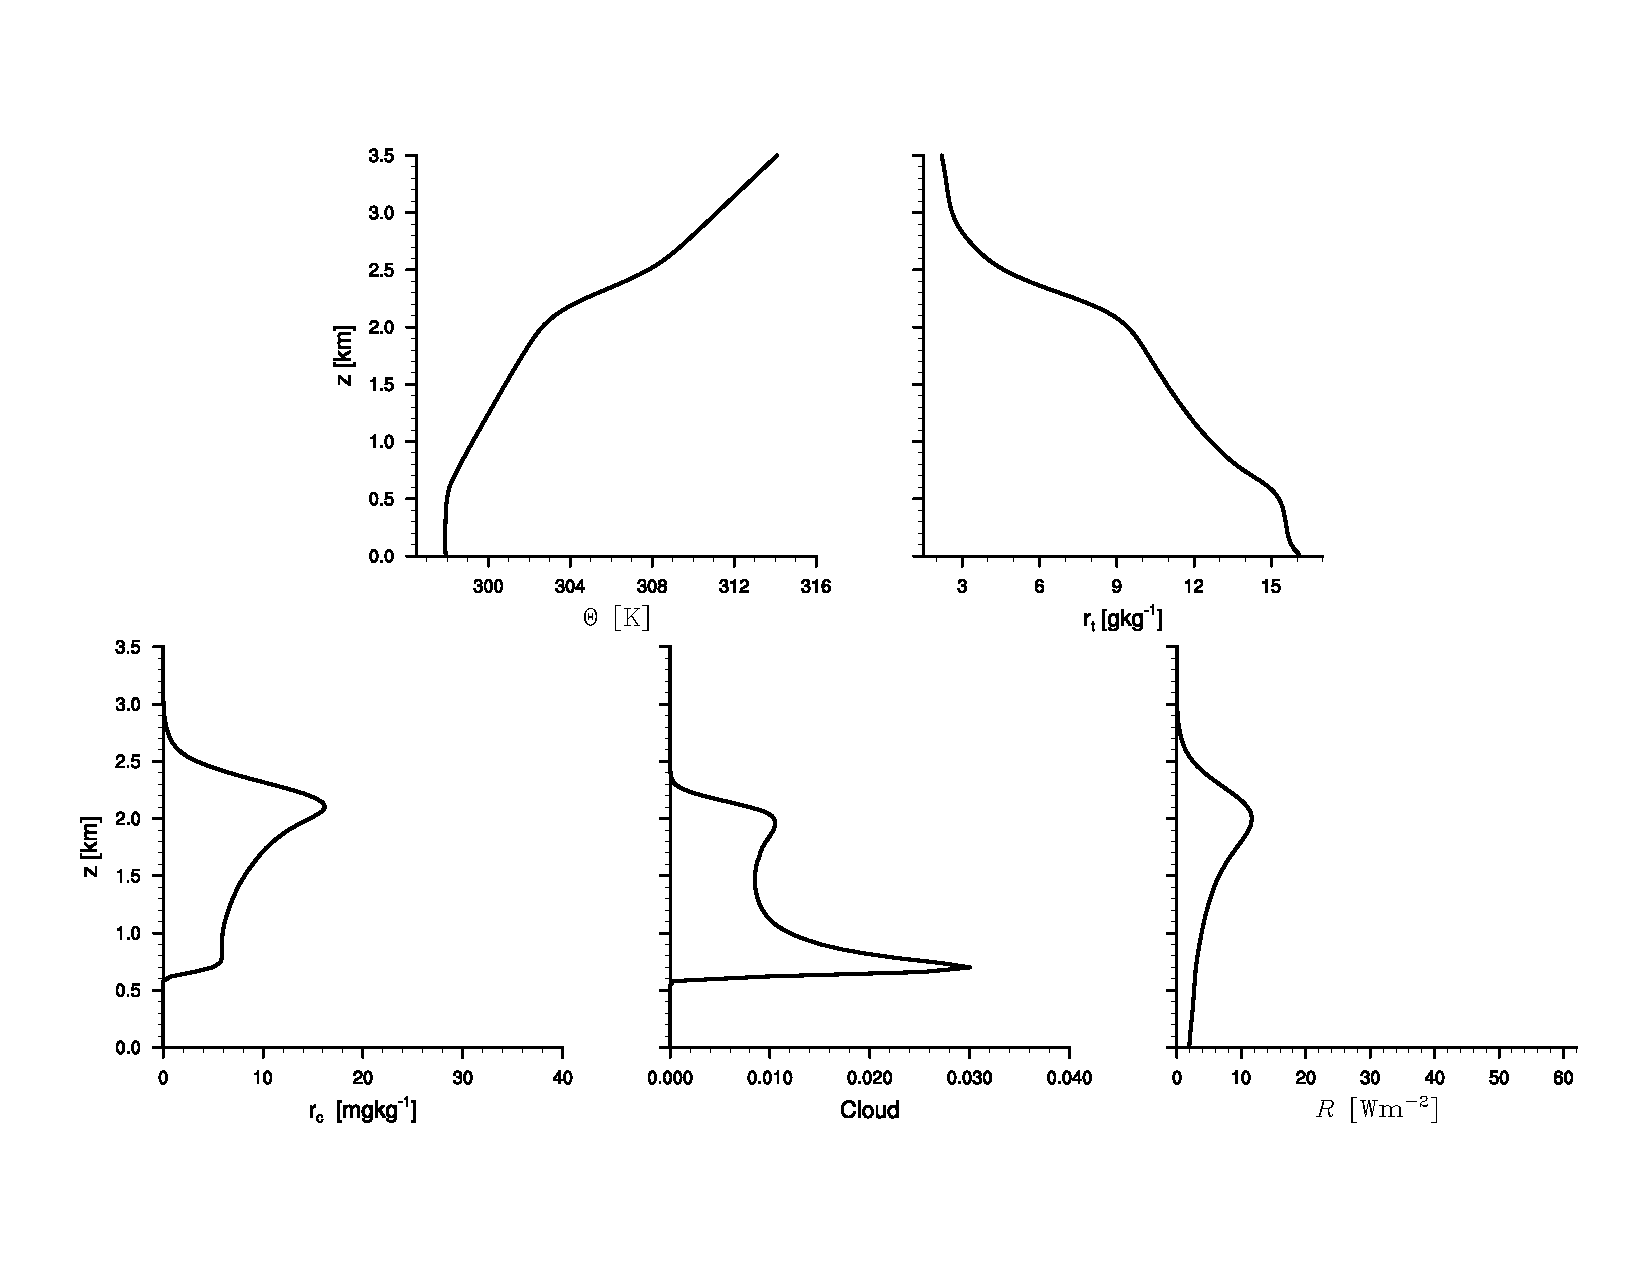
\includegraphics[width=10cm]{rico}
\caption{Thermodynamic profiles showing $\theta_l,$ $r_t,$ $r_c,$ core
cloud fraction and rain rate (in energetic units) averaged over the
last four hours of a 24 hour simulation.}
\label{fig:rico}
\end{figure}

\subsection{Dry CBL}

\begin{figure}
\centering \leavevmode 
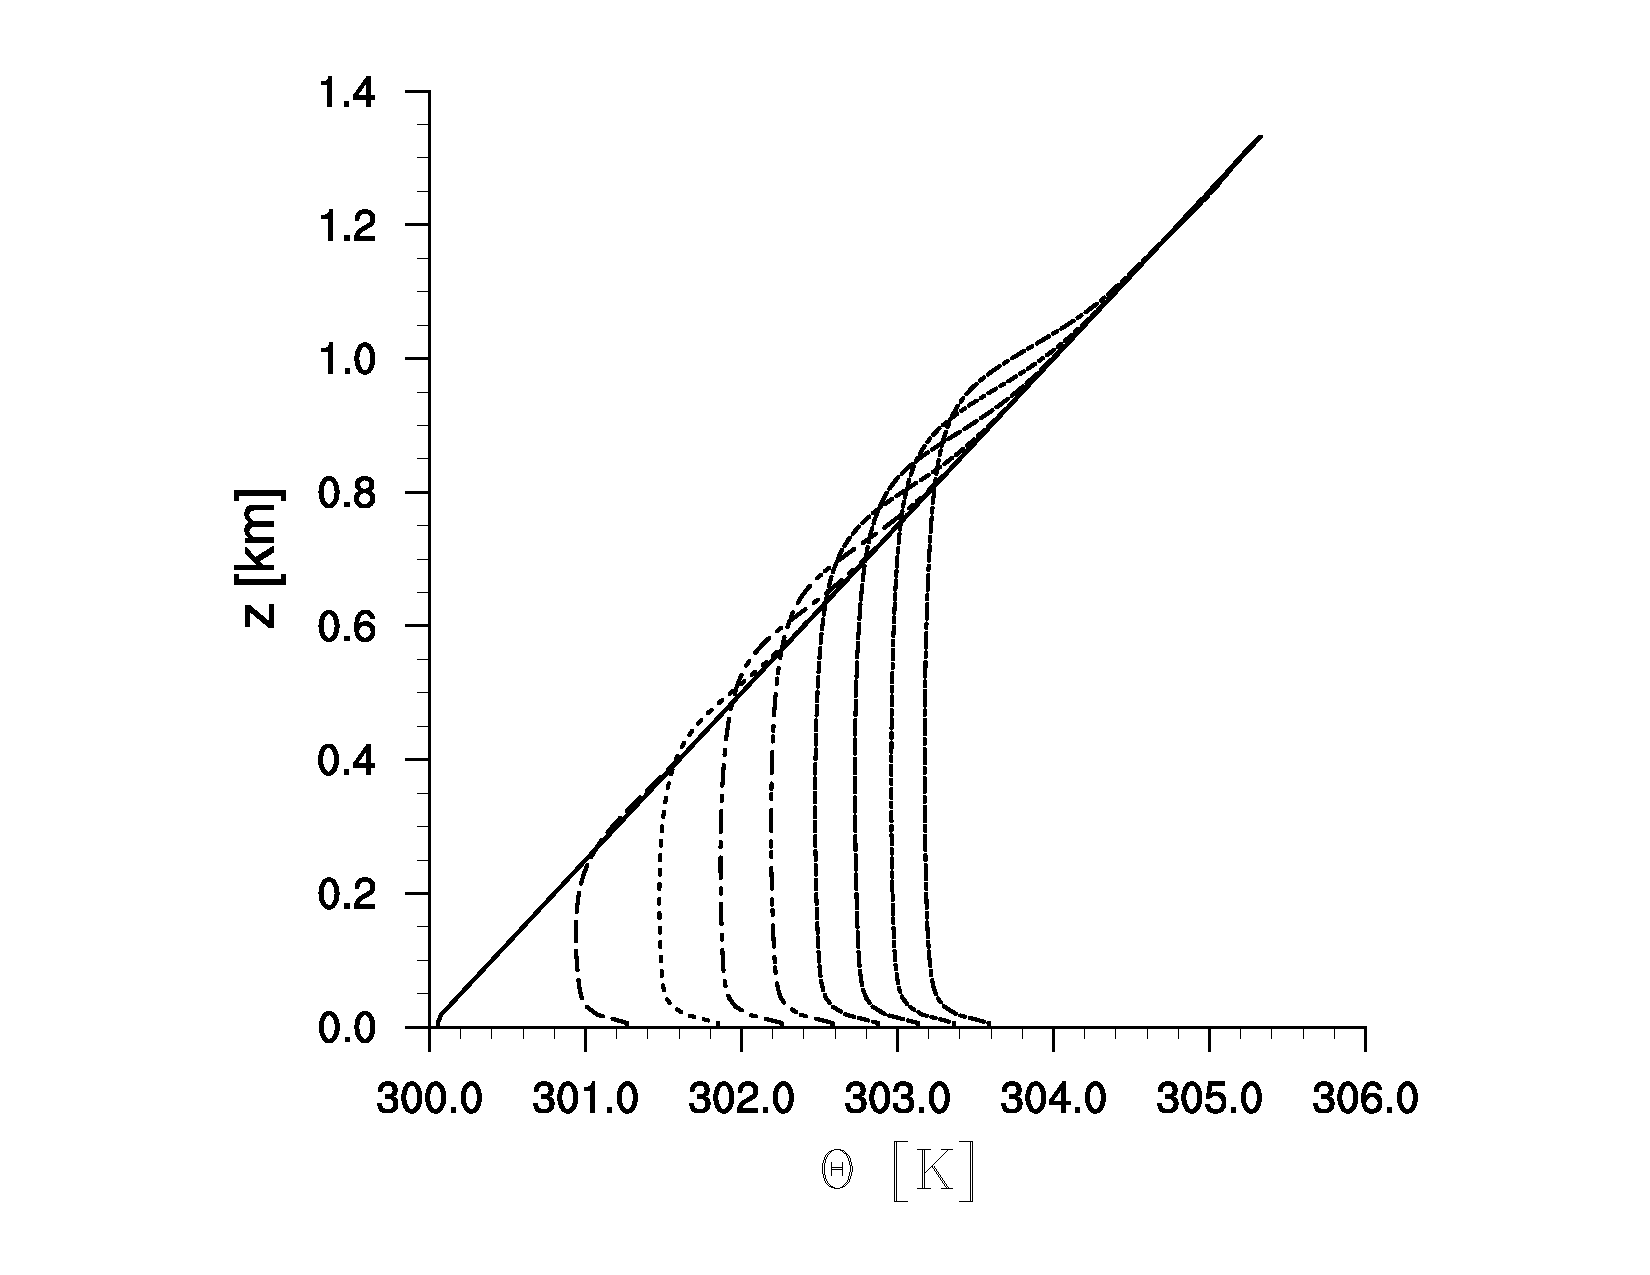
\includegraphics[width=8cm]{cbl}
\caption{Mean potential temperature profile for sample (default) dry
convective boundary layer simulation.  Profiles show averages over
15 minutes plotted at 30 min intervals, with initial state 
(actually state at the end of the first timestep) shown by solid line.}
\label{fig:cbl}
\end{figure}

To run this case we used the NAMELIST
file from the \emph{misc/original} directory. The run was
performed on the IBM power5 BlueVista Machine. It took
less than an hour to finish four hours of simulated time.
The evolution of this run is shown in Figure \ref{fig:cbl} by the
profiles of $\theta$ at half hour intervals, where each profile is a
15 minute average.

\subsection{Smoke} 

\begin{figure}
\centering \leavevmode 
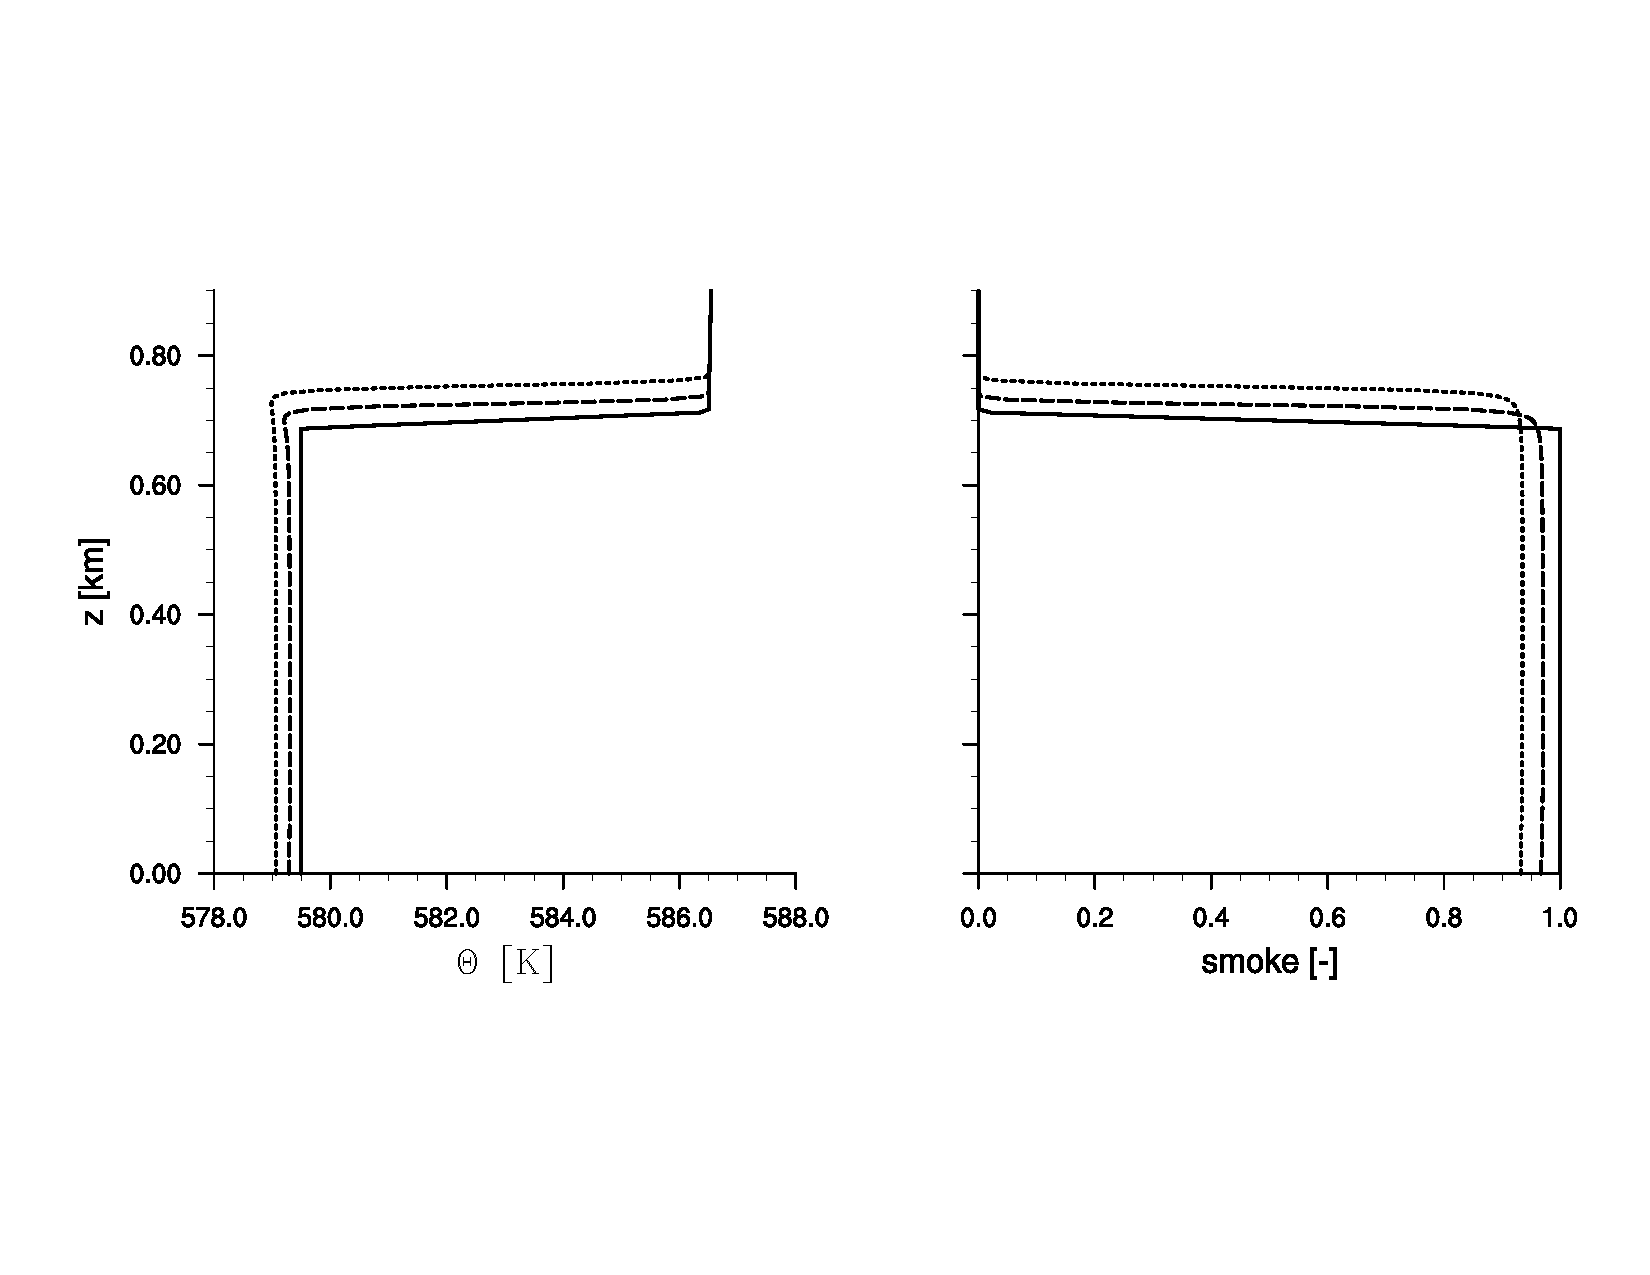
\includegraphics[width=12cm]{smoke}
\caption{Mean potential temperature profile for smoke cloud
simulation.  Shown are profiles of $\theta $ and smoke concentration
averaged over 30 minutes plotted at 2 hr intervals, with initial state
(actually state at the end of the first timestep) shown by solid
line.}
\label{fig:smoke}
\end{figure}

Finally in Figure \ref{fig:smoke} we show the evolution of the smoke
cloud case. For this plot we show the half hour averaged profiles for
the periods ending at 2 and 4 hrs. The initial state is also shown by
the solid line. What we see in the mean profiles is the expected
propagation of the smoke layer into the overlying fluid, accompanied
by the dilution of the smoke layer.  The slight instability at the top
of the smoke layer ($\theta$ decreasing with height) is the signature
of the radiative cooling active in this case.
\newpage
\begin{thebibliography}{8}
\expandafter\ifx\csname natexlab\endcsname\relax\def\natexlab#1{#1}\fi
\expandafter\ifx\csname url\endcsname\relax
  \def\url#1{{\tt #1}}\fi
\expandafter\ifx\csname urlprefix\endcsname\relax\def\urlprefix{URL }\fi
\expandafter\ifx\csname doiprefix\endcsname\relax\def\doiprefix{doi:}\fi

\bibitem[{Cotton(1972)}]{Cotto:1972}
Cotton, W.~R., 1972: Numerical simulation of precipitation development in
  supercooled cumuli-part {I}. {\it Mon. Wea. Rev.\/}, {\bf 100}, 757--763.

\bibitem[{Long(1974)}]{Long:1974}
Long, A.~B., 1974: Solutions to the droplet coalescence equation for polynomial
  kernels. {\it J. Atmos. Sci.\/}, {\bf 31}, 1040.
  
\bibitem[{Heus(2010)}]{Heus:2010}
Heus, T. and van Heerwaarden, C. C. and Jonker, H. J. J. and Pier Siebesma, 
a. and Axelsen, S. and van den Dries, K. and Geoffroy, O. and Moene, a. F. and
Pino, D. and de Roode, S. R. and Vil\`{a}-Guerau de Arellano, J., 2010:
Formulation of the Dutch Atmospheric Large-Eddy Simulation (DALES)
and overview of its applications. {\it Geoscientific Model Development\/}, {\bf 3}, 415-444.

\bibitem[{L\"upkes et~al.(1989)L\"upkes, Beheng, and Doms}]{Lupke:1989}
L\"upkes, C., K.~D. Beheng, and G.~Doms, 1989: A parameterization scheme
  simulating warm rain formation due to collision/coalescence of water drops.
  {\it Contributions to Atmospheric Physics\/}, {\bf 62}, 289--306.

\bibitem[{Milbrandt and Yau(2005)}]{Milbr:2005}
Milbrandt, J.~A. and M.~Yau, 2005: A multimoment bulk microphysics
  parameterization. part {I}: analysis of the role of the spectral shape
  parameter. {\it J. Atmos. Sci.\/}, {\bf 62}, 3051--3064.

\bibitem[{Ogura and Phillip(1962)}]{Ogura:1962}
Ogura, Y.\ and  N.\ A.\ Phillips, 1962: Scale Analysis of Deep and Shallow Convection in the Atmosphere. {\it J.\ Atmos.\ Sci.\/}, {\bf 19}, 173--179.

\bibitem[{Pincus and Stevens(2009)}]{Pincus:2009}
Pincus, R.\ and B.\ Stevens, 2009: Monte Carlo Spectral Integration: a Consistent Approximation for Radiative Transfer in Large Eddy Simulations. {\it Journal of Advances in Modeling Earth Systems\/},
  {\bf 1}.

\bibitem[{Seifert and Beheng(2001)}]{Seife:2001}
Seifert, A. and K.~D. Beheng, 2001: A double-moment parameterization for
  simulating autoconversion, accretion and self collection. {\it Atmos Res\/},
  {\bf 59-60}, 265--281.

\bibitem[{Seifert (2008)}]{Seife:2008}
Seifert, A., 2008: On the Parameterization of Evaporation of Raindrops as
Simulated by a One-Dimensional Rainshaft Model. {\it J. Atmos. Sci.\/},
  {\bf 65}, 3608--3619.

\bibitem[{Stevens et~al.(2005)Stevens, Moeng, Ackerman, Bretherton, Chlond,
  de~Roode, Edwards, Golaz, Jiang, Khairoutdinov, Kirkpatrick, Lewellen, Lock,
  M\"uller, Stevens, Whelan, and Zhu}]{Me:2005b}
Stevens, B., C.-H. Moeng, A.~S. Ackerman, C.~S. Bretherton, A.~Chlond,
  S.~de~Roode, J.~Edwards, J.-C. Golaz, H.~Jiang, M.~Khairoutdinov, M.~P.
  Kirkpatrick, D.~C. Lewellen, A.~Lock, F.~M\"uller, D.~E. Stevens, E.~Whelan,
  and P.~Zhu, 2005: Evaluation of large-eddy simulations via observations of
  nocturnal marine stratocumulus. {\it Mon. Wea. Rev.\/}, {\bf 133},
  1443--1462.

\bibitem[{Stevens et~al.(1999)Stevens, Moeng, and Sullivan}]{Me:1999a}
Stevens, B., C.-H. Moeng, and P.~P. Sullivan, 1999: Large-eddy simulations of
  radiatively driven convection: sensitivities to the representation of small
  scales. {\it J. Atmos. Sci.\/}, {\bf 56}, 3963--3984.

\bibitem[{Stevens and Seifert(2008)}]{Me:2008}
Stevens, B. and A.~Seifert, 2008: On the sensitivity of simulations of shallow
  cumulus convection to their microphysical representation. {\it J. Meteorol.
  Soc. Japan\/}.

\end{thebibliography}

\end{document}












